
\subsection{Resultats}

Per la simulació de la transferència de calor, es discretitza uniformement en $N_1 = 30$ volums de control, la qual dona lloc a $3844$ nodes de control. Com s'ha vist en la secció \ref{sec:analisi_pas_de_temps}, un pas de temps de $\Delta t = 10.00 \ \second$ amb un esquema de Crank--Nicolson és adient. Pel mètode de Gauss--Seidel es pren un criteri de convergència $\delta = 10^{-11}$.  

A continuació es mostren els resultats donats pel codi de simulació. A la figura \ref{fig:nous_1} es mostren els mapes de temperatura entre $t = 1000 \ \second$ i $t = 6000 \ \second$, cada $1000 \ \second$. A la figura \ref{fig:nous_2} es mostren alguns mapes de temperatura entre $t = 7000 \ \second$ i $t = 20000 \ \second$. S'observa que la temperatura segueix una distribució radial des del centre del domini d'estudi. Les zones amb un refredament més ràpid són les cantonades a causa de la major superfície de transferència de calor.

\begin{figure}[ht]
	\centering
	\begin{subfigure}{.5\textwidth}
		\centering
		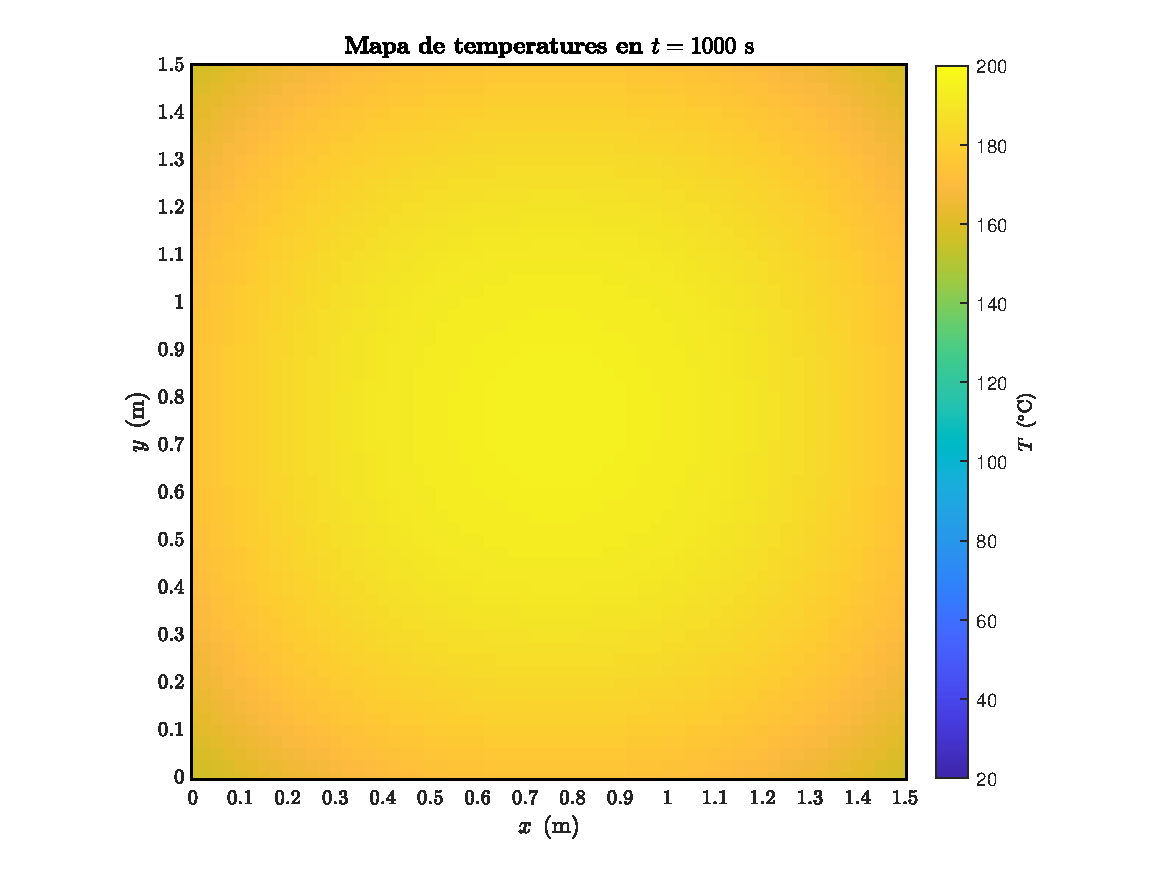
\includegraphics[width=.95\linewidth]{imagenes/06_canvi_condicions_contorn/t_1000.pdf}
		\vspace{-10pt}
		\caption{Mapa de temperatures per $t = 1000 \ \second$.}
		\label{fig:nou_t_1000}
	\end{subfigure}%
	\begin{subfigure}{.5\textwidth}
		\centering
		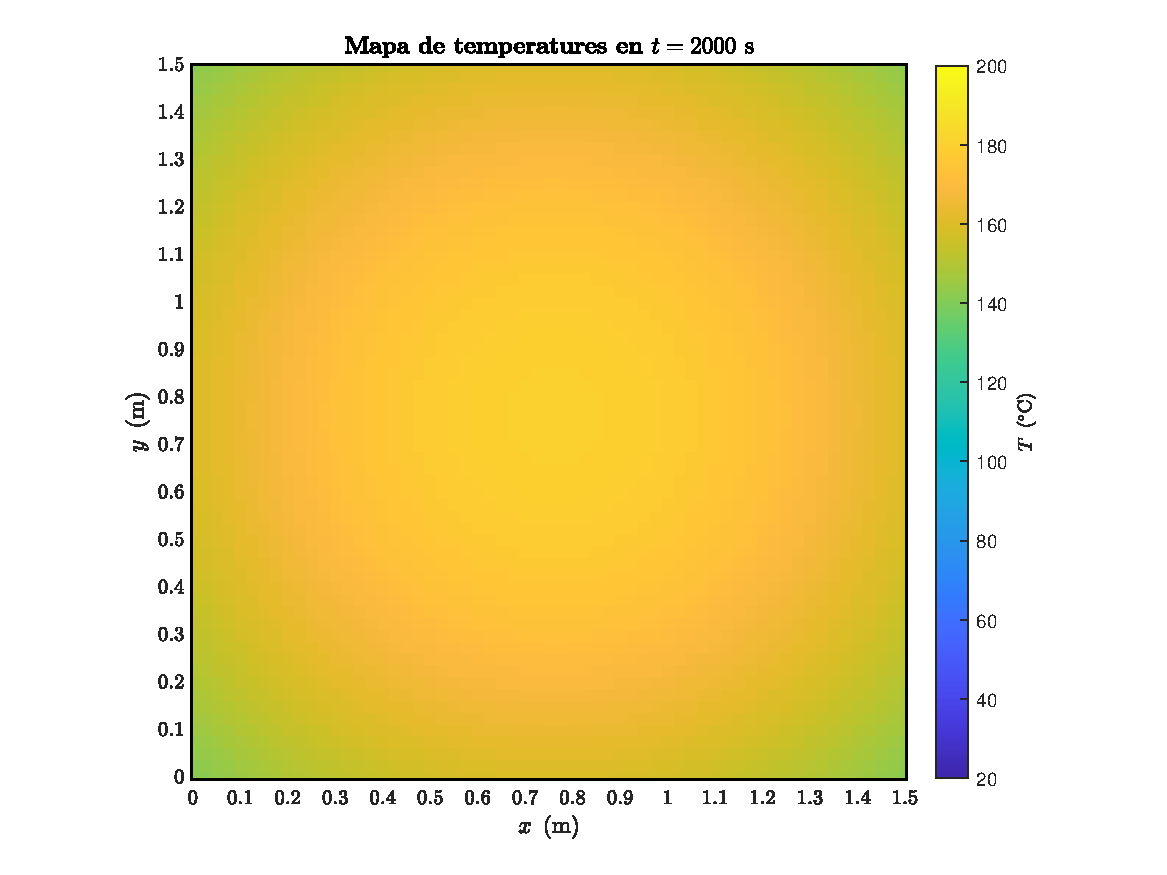
\includegraphics[width=.95\linewidth]{imagenes/06_canvi_condicions_contorn/t_2000.pdf}
		\vspace{-10pt}
		\caption{Mapa de temperatures per $t = 2000 \ \second$.}
		\label{fig:nou_t_2000}
	\end{subfigure}
	\begin{subfigure}{.5\textwidth}
		\centering
		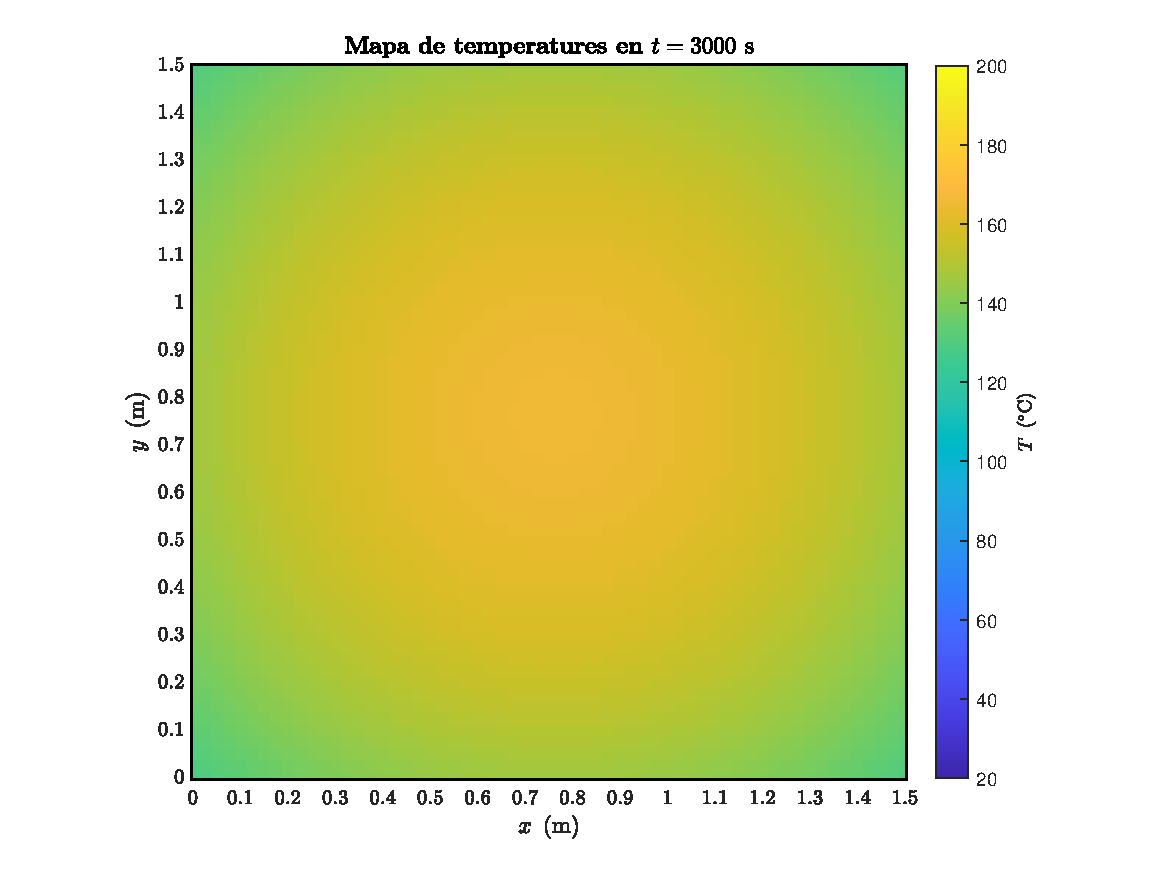
\includegraphics[width=.95\linewidth]{imagenes/06_canvi_condicions_contorn/t_3000.pdf}
		\vspace{-10pt}
		\caption{Mapa de temperatures per $t = 3000 \ \second$.}
		\label{fig:nou_t_3000}
	\end{subfigure}%
	\begin{subfigure}{.5\textwidth}
		\centering
		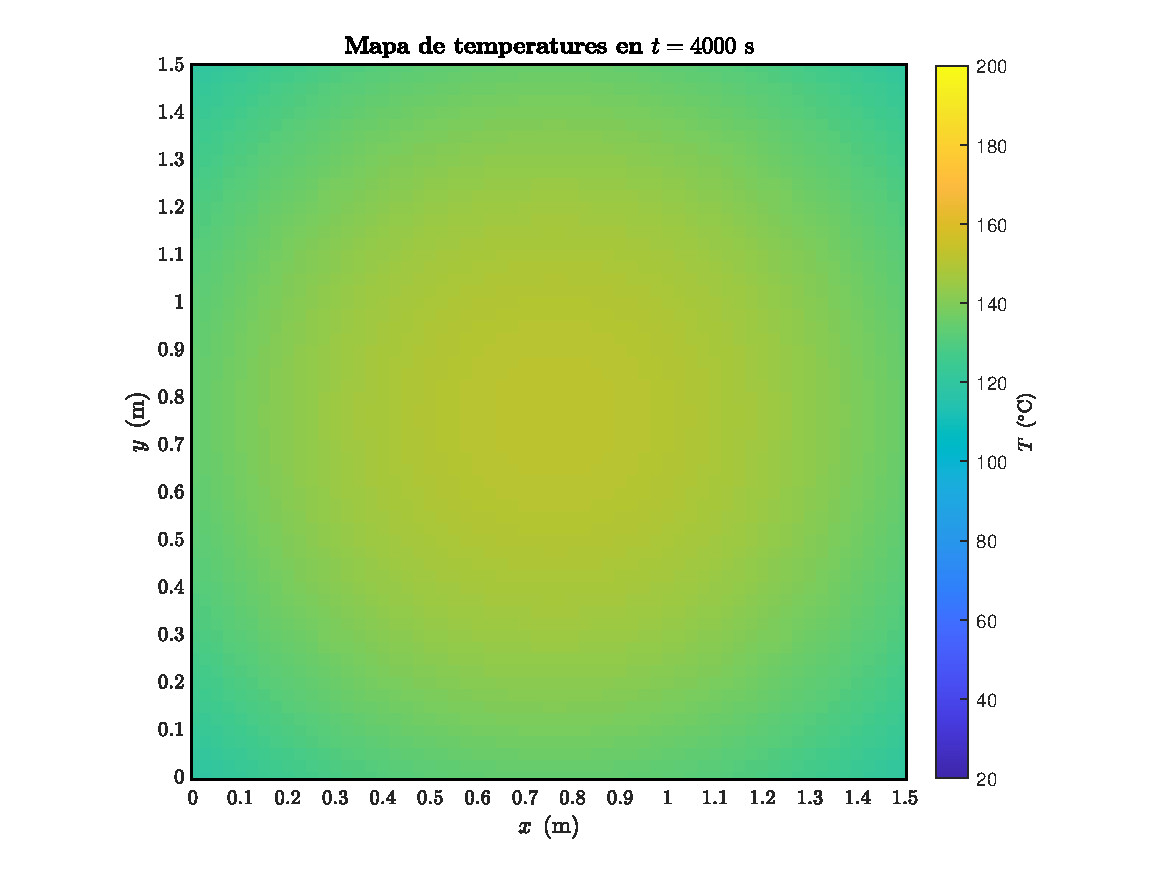
\includegraphics[width=.95\linewidth]{imagenes/06_canvi_condicions_contorn/t_4000.pdf}
		\vspace{-10pt}
		\caption{Mapa de temperatures per $t = 4000 \ \second$.}
		\label{fig:nou_t_4000}
	\end{subfigure}
	\begin{subfigure}{.5\textwidth}
		\centering
		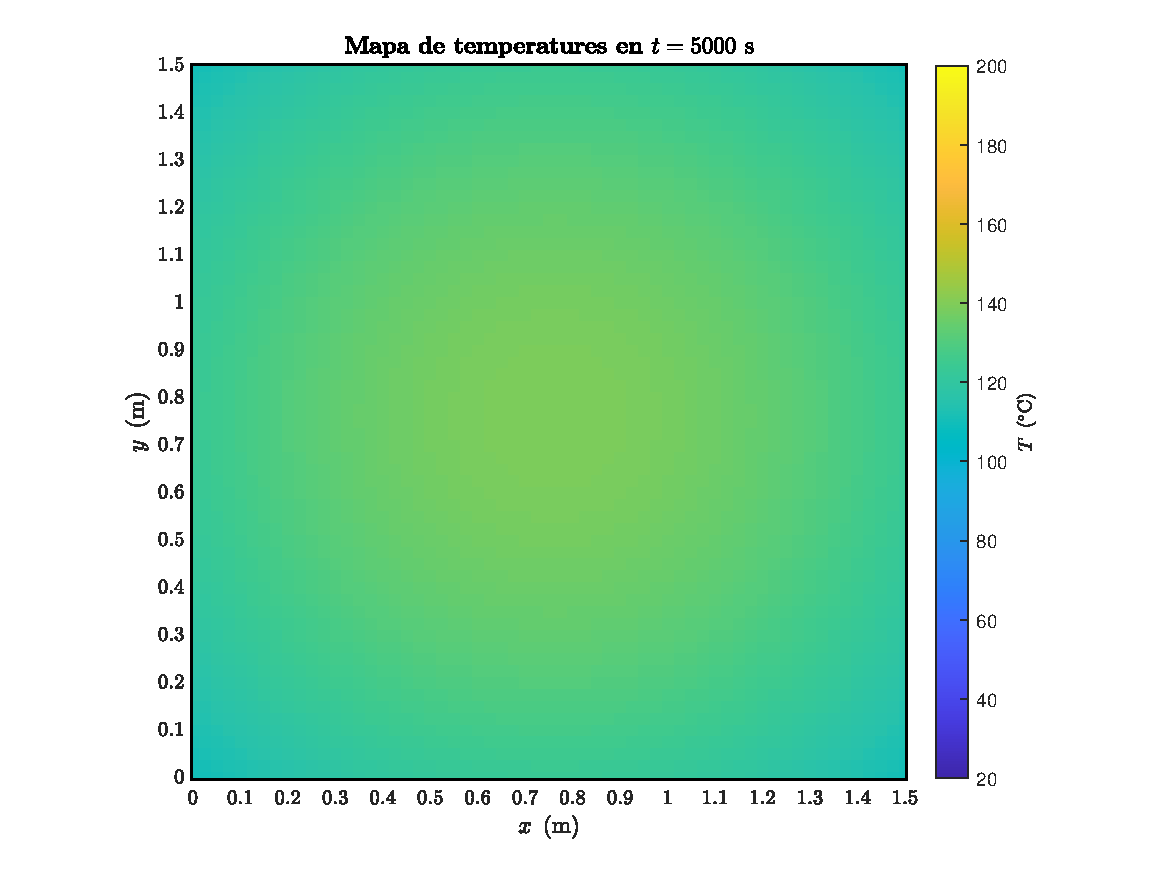
\includegraphics[width=.95\linewidth]{imagenes/06_canvi_condicions_contorn/t_5000.pdf}
		\vspace{-10pt}
		\caption{Mapa de temperatures per $t = 5000 \ \second$.}
		\label{fig:nou_t_5000}
	\end{subfigure}%
	\begin{subfigure}{.5\textwidth}
		\centering
		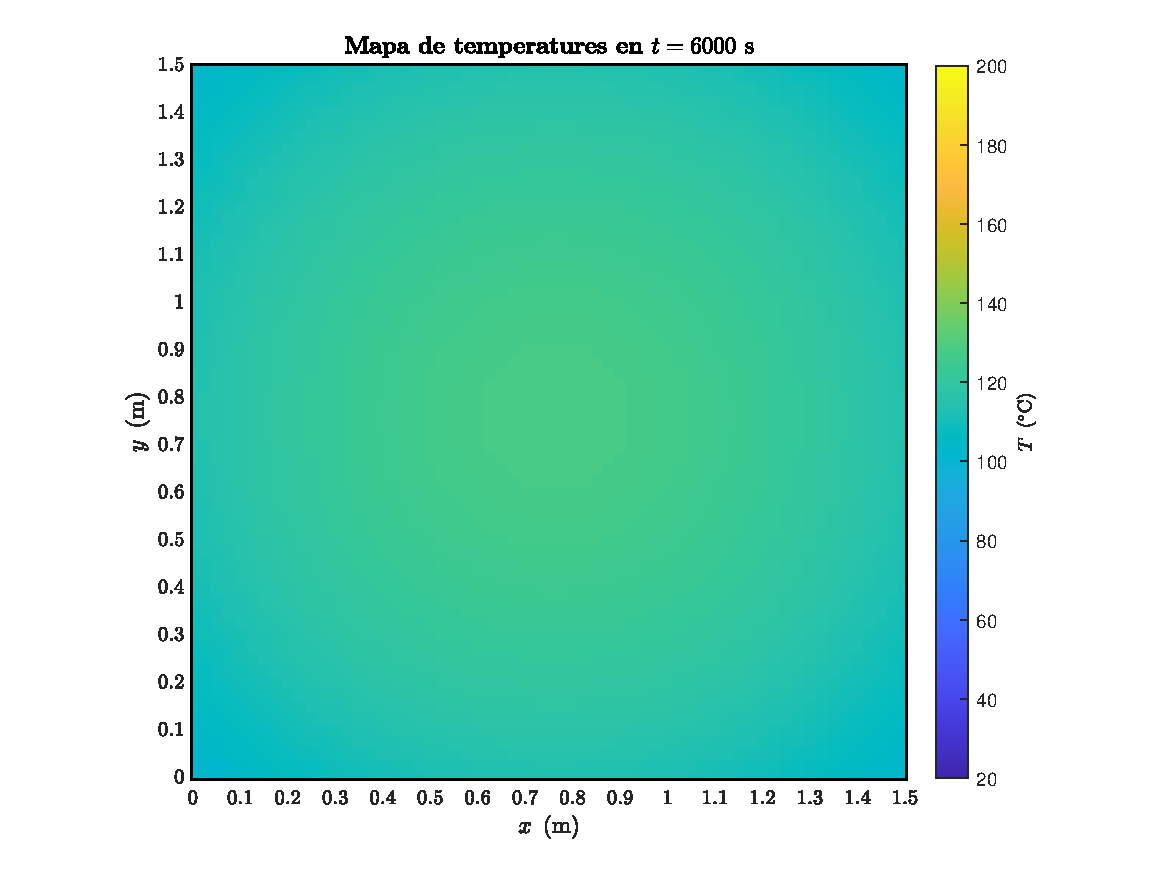
\includegraphics[width=.95\linewidth]{imagenes/06_canvi_condicions_contorn/t_6000.pdf}
		\vspace{-10pt}
		\caption{Mapa de temperatures per $t = 6000 \ \second$.}
		\label{fig:nou_t_6000}
	\end{subfigure}
	\caption{Mapes de temperatures del nou cas entre $t = 1000 \ \second$ i $t = 6000 \ \second$, amb discretitzacions uniformes de $N_1 = 30$ nodes. Pas de temps $\Delta = 10.00 \ \second$, esquema Crank--Nicolson i sense interpolació. L'escala de temperatures és entre $20 \ \celsius$ i $200 \ \celsius$.}
	\label{fig:nous_1}
\end{figure} 

\begin{figure}[ht]
	\centering
	\begin{subfigure}{.5\textwidth}
		\centering
		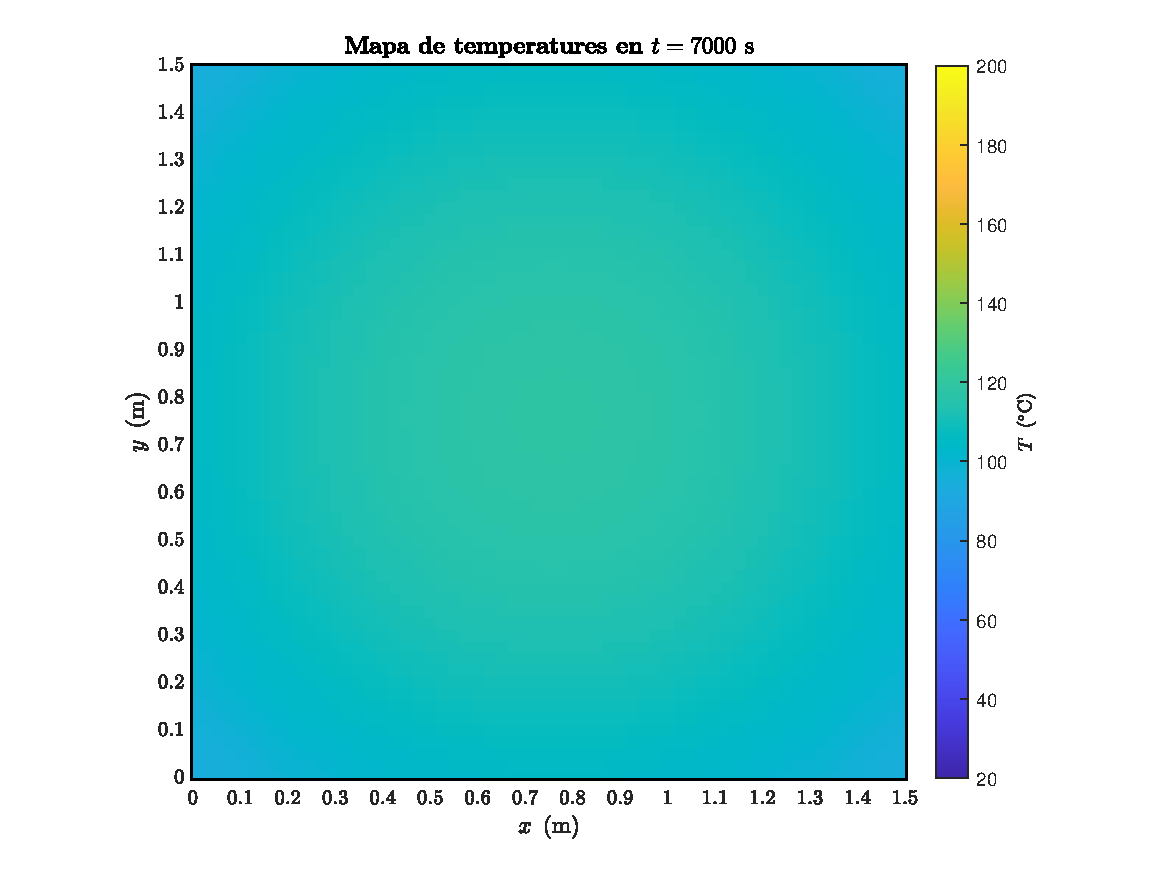
\includegraphics[width=.95\linewidth]{imagenes/06_canvi_condicions_contorn/t_7000.pdf}
		\vspace{-10pt}
		\caption{Mapa de temperatures per $t = 7000 \ \second$.}
		\label{fig:nou_t_7000}
	\end{subfigure}%
	\begin{subfigure}{.5\textwidth}
		\centering
		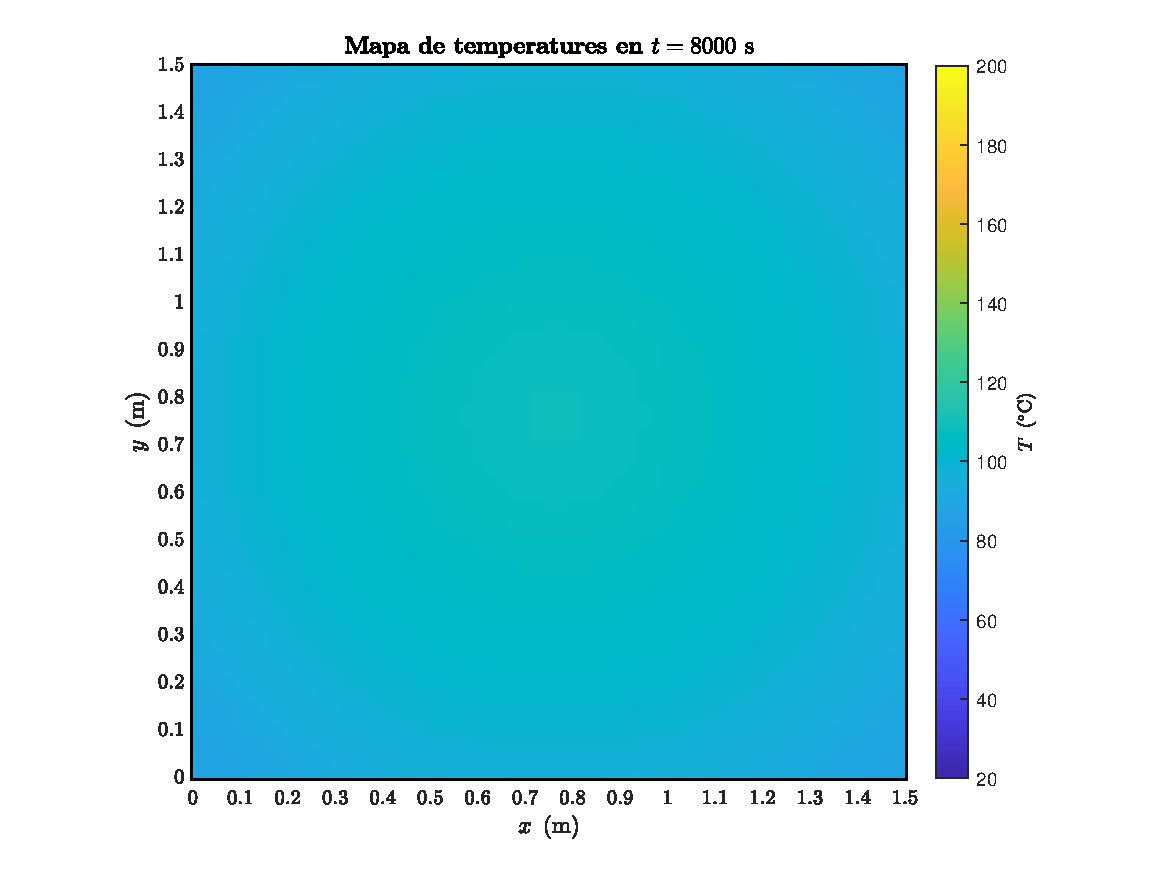
\includegraphics[width=.95\linewidth]{imagenes/06_canvi_condicions_contorn/t_8000.pdf}
		\vspace{-10pt}
		\caption{Mapa de temperatures per $t = 8000 \ \second$.}
		\label{fig:nou_t_8000}
	\end{subfigure}
	\begin{subfigure}{.5\textwidth}
		\centering
		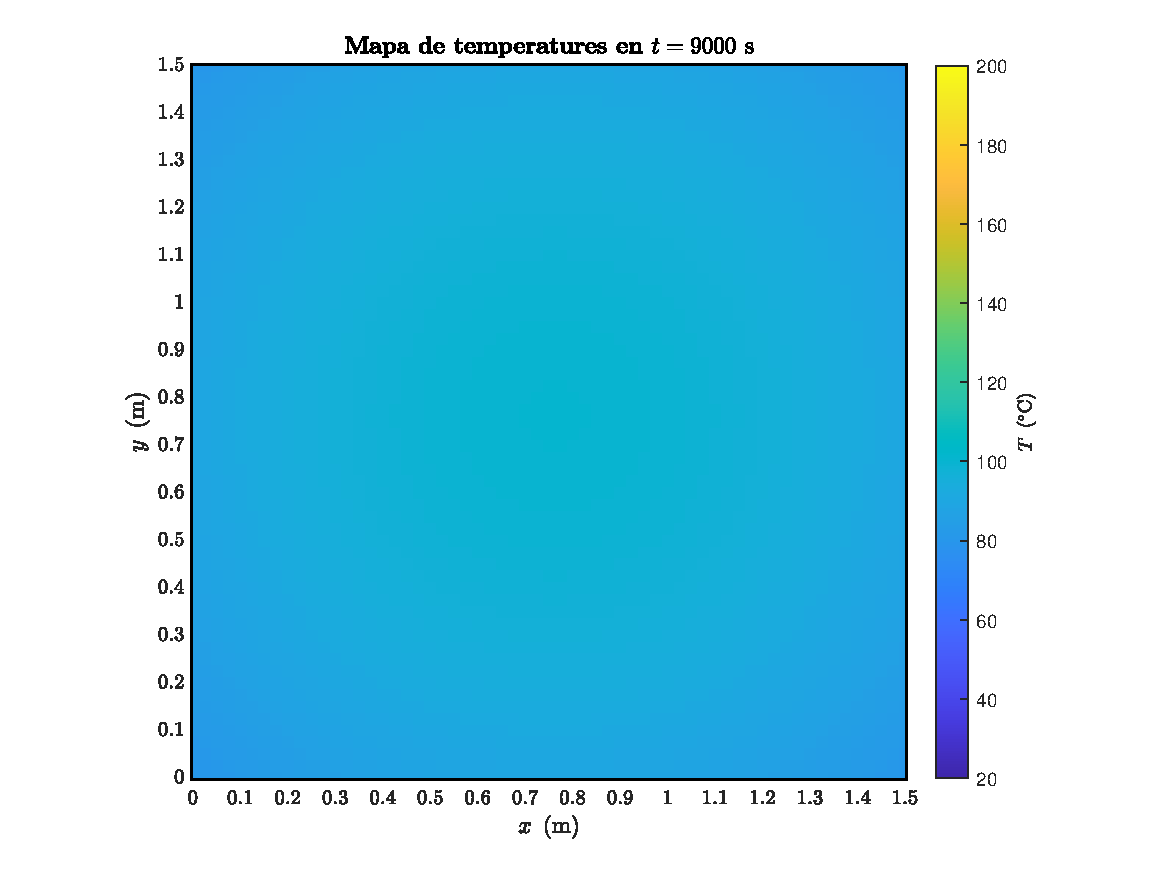
\includegraphics[width=.95\linewidth]{imagenes/06_canvi_condicions_contorn/t_9000.pdf}
		\vspace{-10pt}
		\caption{Mapa de temperatures per $t = 9000 \ \second$.}
		\label{fig:nou_t_9000}
	\end{subfigure}%
	\begin{subfigure}{.5\textwidth}
		\centering
		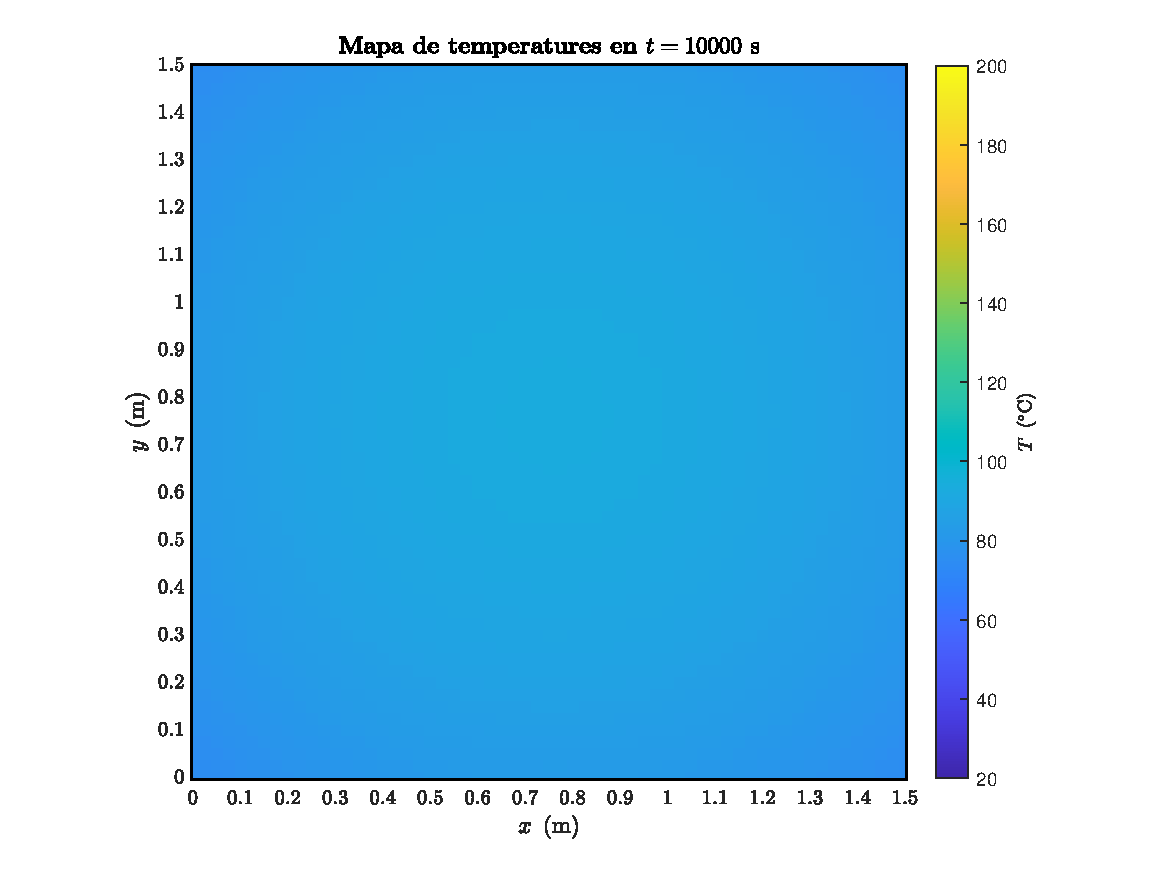
\includegraphics[width=.95\linewidth]{imagenes/06_canvi_condicions_contorn/t_10000.pdf}
		\vspace{-10pt}
		\caption{Mapa de temperatures per $t = 10000 \ \second$.}
		\label{fig:nou_t_10000}
	\end{subfigure}
	\begin{subfigure}{.5\textwidth}
		\centering
		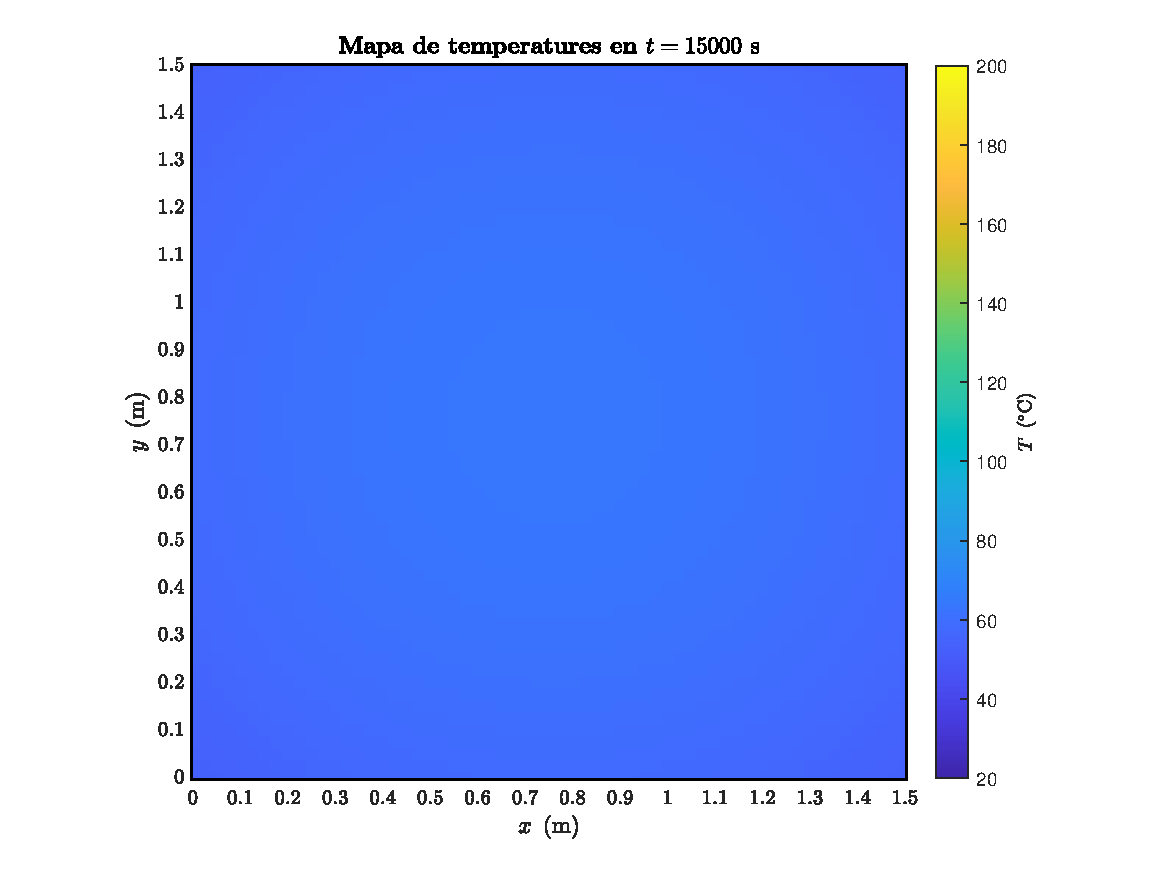
\includegraphics[width=.95\linewidth]{imagenes/06_canvi_condicions_contorn/t_15000.pdf}
		\vspace{-10pt}
		\caption{Mapa de temperatures per $t = 15000 \ \second$.}
		\label{fig:nou_t_15000}
	\end{subfigure}%
	\begin{subfigure}{.5\textwidth}
		\centering
		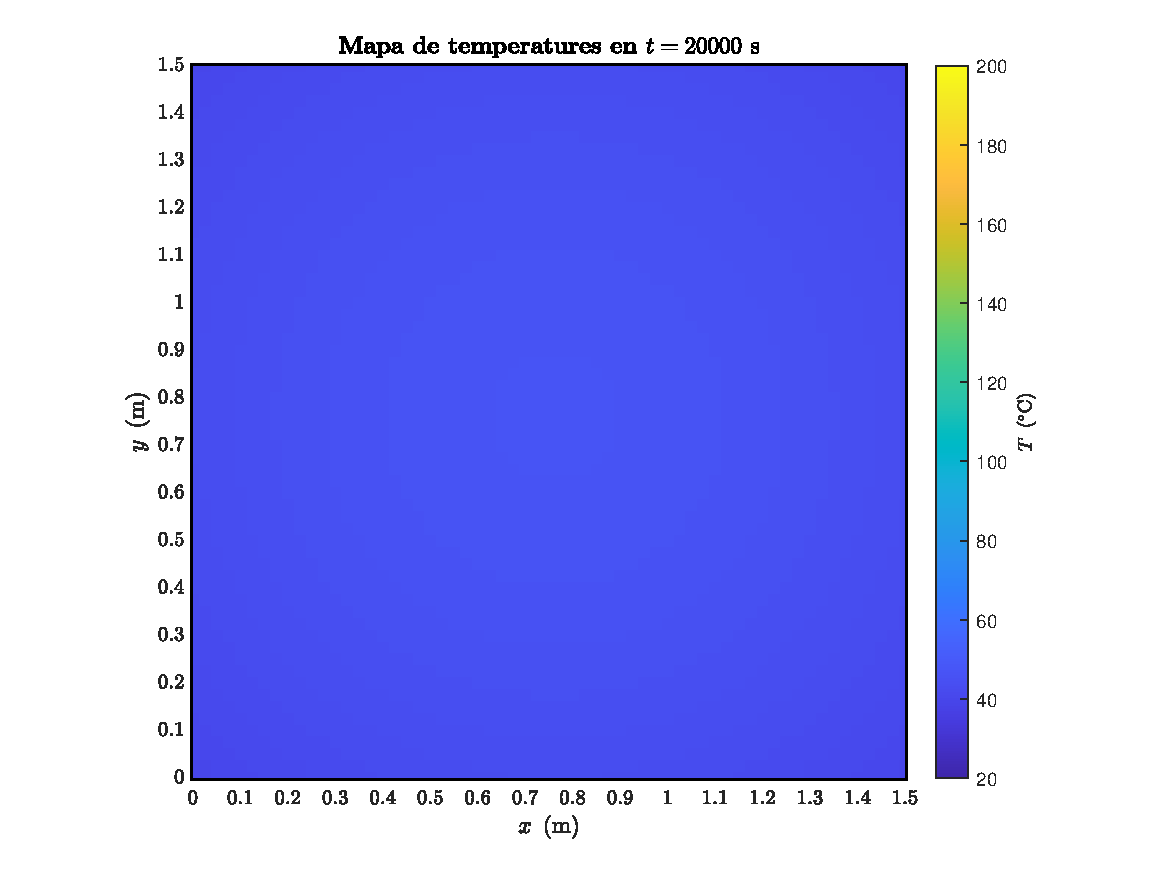
\includegraphics[width=.95\linewidth]{imagenes/06_canvi_condicions_contorn/t_20000.pdf}
		\vspace{-10pt}
		\caption{Mapa de temperatures per $t = 20000 \ \second$.}
		\label{fig:nou_t_20000}
	\end{subfigure}
	\caption{Mapes de temperatures del nou cas entre $t = 7000 \ \second$ i $t = 20000 \ \second$, amb discretitzacions uniformes de $N_1 = 30$ nodes. Pas de temps $\Delta = 10.00 \ \second$, esquema Crank--Nicolson i sense interpolació. L'escala de temperatures és entre $20 \ \celsius$ i $200 \ \celsius$.}
	\label{fig:nous_2}
\end{figure} 
